\documentclass[landscape]{article}
\usepackage[pdftex]{graphicx}
\pagestyle{empty}
\oddsidemargin  -0.5 in
\evensidemargin -0.5 in
\headheight     0 in
\topmargin      -1 in
\textheight     7.7 in
\textwidth      10 in
\begin{document}
\huge
\renewcommand{\labelitemi}{-}
\setlength{\parindent}{0 cm}

\mbox{ }

\vfill

\mbox{ }

\vfill

\begin{center}
  Bounding the Trigger Inefficiency for $\Upsilon(1,2,3S)$

  \vfill

  Jim Pivarski
\end{center}

\vfill

\mbox{ }

\vfill

\mbox{ }

\pagebreak

\mbox{ }

\vfill

First cut in any analysis: the trigger

\vfill

Problem: only events which {\it pass} the trigger can be compared with
data

\vfill

My trigger lines: ``Hadron'' OR ``RadTau'' OR ``ElTrack''

\vfill

MC efficiency for these lines is 99.5\% (nicely bounded above)

\vfill

Is the MC generating {\it too few} untriggered events?

\vfill

\mbox{ }

\pagebreak

\mbox{ }

\vfill

My trigger lines: ``Hadron'' OR ``RadTau'' OR ``ElTrack''

\vspace{0.5 cm}

Trigger depends on four variables: $\begin{array}{c} \\ \underbrace{\mbox{\#CBLO, \#CBMD,}} \\ \mbox{CC cluster counting} \end{array} \begin{array}{c} \\ \underbrace{\mbox{\#AXIAL, \#STEREO}} \\ \mbox{DR track counting} \end{array}$

\vfill

STEP 1: Check CC cluster counting with ``TwoTrack'' trigger line

\vspace{1 cm}
STEP 2: Quantify systematic error from uncertainty in trigger
track-finding efficiency

\vspace{1 cm}
STEP 3.1: Check MC reconstructed track distribution with
$\Upsilon(2S) \to \Upsilon(1S)$ cascade

\vspace{1 cm}
STEP 3.2: Quantify systematic error from uncertainty in number of
0-, 1-track events

\vspace{1 cm}
STEP 3.3: Quantify systematic error from differences in
reconstructed track efficiency between data and MC

\vfill

\pagebreak

\vspace{1 cm}

{\bf STEP 1: Check CC cluster counting with ``TwoTrack'' trigger}

\vfill

P($\Upsilon$ passes trigger $|$ TwoTrack) = P(event passes trigger $|$ TwoTrack and event is $\Upsilon$)

\vfill

These cuts guarantee negligible backgrounds and no lower bounds on CC quantities:

\vspace{0.5 cm}

%%%%%%%%%%% charged energy cut reduces efficiency from 96% to 81%
\begin{center}
  \begin{tabular}{l l}
    data: TwoTrack trigger & \hspace{-0.4 cm} AND analysis cuts AND charged energy $>$ 35\% COM \\
    & \hspace{-0.4 cm} AND continuum-subtraction
  \end{tabular}

  \medskip
  \begin{tabular}{l}
    MC: TwoTrack trigger AND analysis cuts AND charged energy $>$ 35\% COM
  \end{tabular}
\end{center}

\vfill

P(passes ``Hadron'' OR ``RadTau'' OR ``ElTrack'' $|$ all those cuts):

\begin{center}
  \renewcommand{\arraystretch}{1.25}
  \begin{tabular}{c c c c}
  \mbox{\hspace{4 cm}} & \mbox{\hspace{2 cm}} $\Upsilon(1S)$ \mbox{\hspace{2 cm}} & \mbox{\hspace{2 cm}} $\Upsilon(2S)$ \mbox{\hspace{2 cm}} & \mbox{\hspace{2 cm}} $\Upsilon(3S)$ \mbox{\hspace{2 cm}} \\\hline
  data & 99.97\% & 99.48\% & 99.51\% \\
  MC & 99.83\% & 99.86\% & 99.86\% \\
  difference & 0.14\% & 0.38\% & 0.35\% \\
  & $\pm$0.20\% & $\pm$0.31\% & $\pm$1.00\%
  \end{tabular}
\end{center}

\pagebreak

\vspace{1 cm}

{\bf STEP 2: Quantify systematic error from uncertainty in trigger
track-finding efficiency}

\vspace{1.5 cm}

Toy MC: 
\begin{enumerate}

  \item pick a random \#reconstructed tracks from the full MC's distribution

  \item for this \#tracks, pick a random \#CBLO, \#CBMD (2-d distributions from full MC)

  \item for this \#tracks, pick a random \#AXIAL (from full MC or from data)

  \item for this \#AXIAL, pick a random \#STEREO (from full MC or from data)

  \item calculate (``Hadron'' OR ``RadTau'' OR ``ElTrack'') and repeat many times

\end{enumerate}

\vfill

\begin{center} 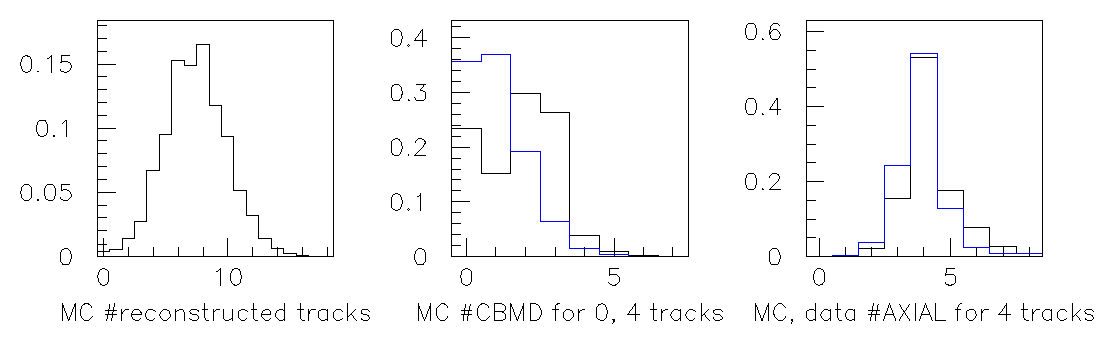
\includegraphics[width=0.9\linewidth]{drawplots.pdf} \end{center}

\vfill

\pagebreak

\vspace{1 cm}

{\bf STEP 2: Quantify systematic error from uncertainty in trigger
track-finding efficiency}

\vspace{1.5 cm}

Toy MC: 
\begin{enumerate}

  \item pick a random \#reconstructed tracks from the full MC's distribution

  \item for this \#tracks, pick a random \#CBLO, \#CBMD (2-d distributions from full MC)

  \item for this \#tracks, pick a random \#AXIAL (from full MC or from data)

  \item for this \#AXIAL, pick a random \#STEREO (from full MC or from data)

  \item calculate (``Hadron'' OR ``RadTau'' OR ``ElTrack'') and repeat many times

\end{enumerate}

\vfill

\begin{center}
  \renewcommand{\arraystretch}{1.25}
  \begin{tabular}{p{12 cm} c c c}
  & \mbox{\hspace{0.5 cm}} $\Upsilon(1S)$ \mbox{\hspace{0.5 cm}} & \mbox{\hspace{0.5 cm}} $\Upsilon(2S)$ \mbox{\hspace{0.5 cm}} & \mbox{\hspace{0.5 cm}} $\Upsilon(3S)$ \mbox{\hspace{0.5 cm}} \\\hline
  Full MC & 99.7\% & 99.4\% & 99.5\% \\
  Toy MC & 99.7\% & 99.5\% & 99.6\% \\
  Get \#AXIAL, \#STEREO from data & 99.6\% & 99.4\% & 99.5\% \\
  Throw out every 12$^{\mbox{\large th}}$ AXIAL track in MC & 99.5\% & 99.4\% & 99.5\% \\
  \end{tabular}
\end{center}
\begin{flushright} (all table uncertainties $<$ 0.03\%) \end{flushright}

\vfill

\pagebreak

\vspace{1 cm}

{\bf STEP 3.1: Check MC reconstructed track distribution with cascade}

\vfill

$\Upsilon(2S) \to \Upsilon(1S) \underbrace{\pi^+\pi^-}$

\hspace{5.5 cm} $\hookrightarrow$ satisfy TwoTrack requirement, L4, and ``quality tracks $\ge$ 2''

\vfill

\begin{tabular}{p{0.4\linewidth} p{0.03\linewidth} p{0.55\linewidth}}
  \begin{minipage}{\linewidth}

  \begin{enumerate}

    \item Get {\bf all} $\Upsilon(2S)$ events from tau subcollection with TwoTrack trigger

    \bigskip
    \item Plot $\pi^+\pi^-$ missing mass distribution for each number of tracks

%%     \item Scale up wrong-sign combinations to match right-sign, using sideband

%%     \item Subtract $\Upsilon(1S)$ mass peak from combinatoric background

    \bigskip
    \item Count number of $\Upsilon(1S)$ events in each peak

    \bigskip
    \item Do exactly the same for MC

    \bigskip
    \item Plot number of $\Upsilon(1S)$ events per number of non-$\pi^+\pi^-$ tracks $\longrightarrow$ $\longrightarrow$ $\longrightarrow$ $\longrightarrow$ $\longrightarrow$ $\longrightarrow$ $\longrightarrow$

  \end{enumerate}

  \end{minipage} & &
  \begin{minipage}{\linewidth} 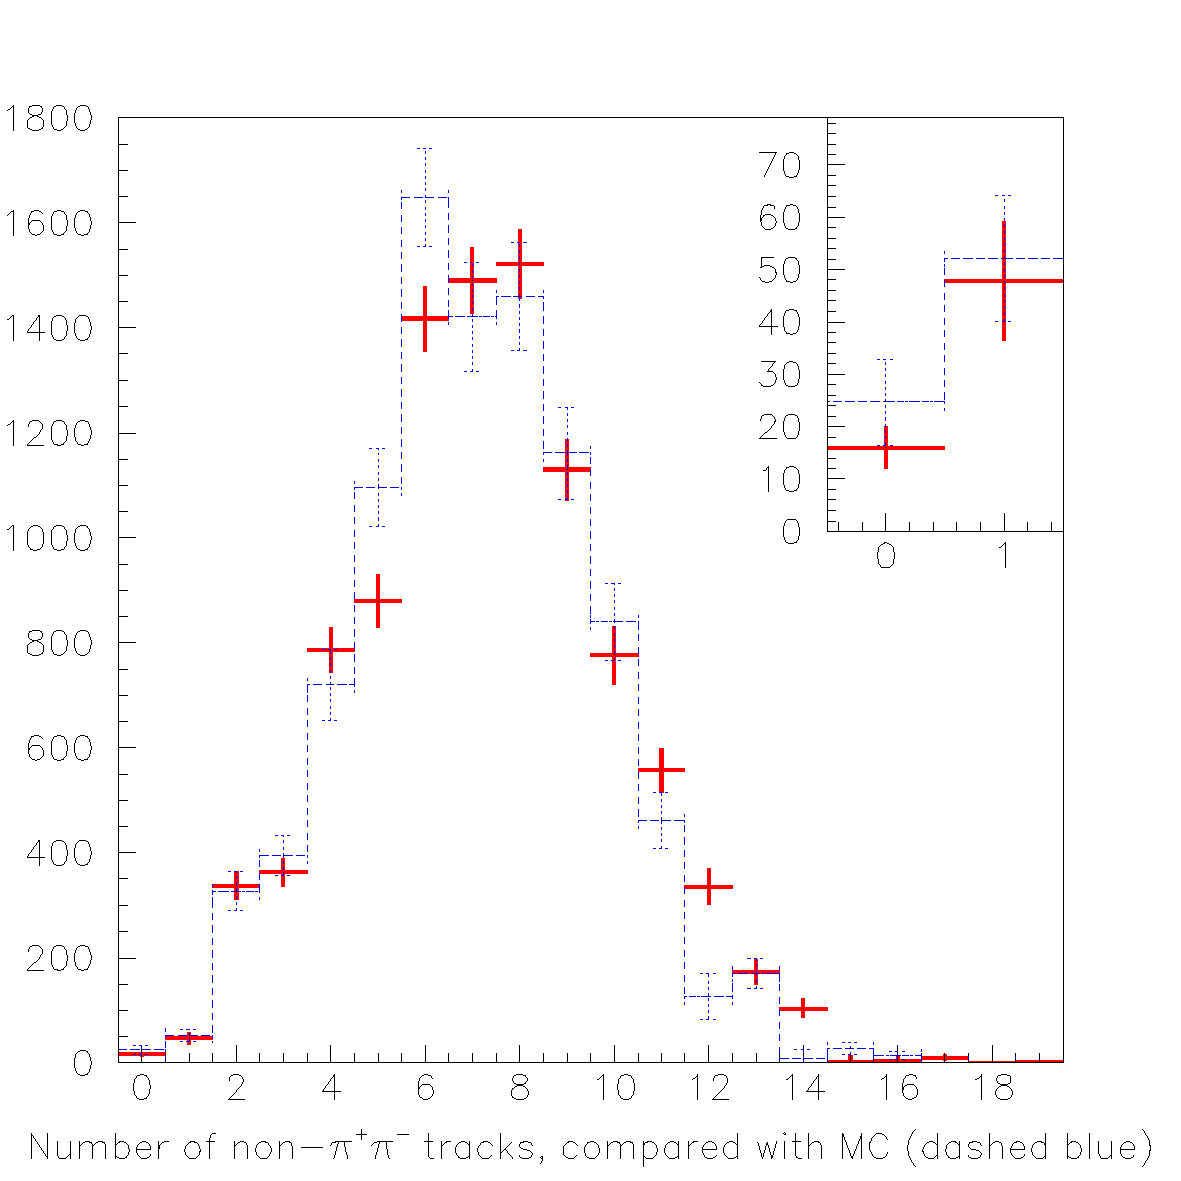
\includegraphics[width=\linewidth]{cascades_tracks_boost3_tt.pdf} \end{minipage}
\end{tabular}

\vfill

\pagebreak

\vspace{1 cm}

{\bf STEP 3.2: Quantify systematic error from uncertainty in number of
0-, 1-track events}

\vfill

Instead of replacing the \#AXIAL and \#STEREO distributions, replace the
\#tracks distribution

\vfill

(For apples-to-apples, we must compare {\it boosted} data to {\it boosted} MC.)

\vfill

\begin{center}
  \renewcommand{\arraystretch}{1.25}
  \begin{tabular}{p{12 cm} c c c}
  & \mbox{\hspace{0.5 cm}} $\Upsilon(1S)$ \mbox{\hspace{0.5 cm}} & \mbox{\hspace{0.5 cm}} $\Upsilon(2S)$ \mbox{\hspace{0.5 cm}} & \mbox{\hspace{0.5 cm}} $\Upsilon(3S)$ \mbox{\hspace{0.5 cm}} \\\hline
  Toy MC & 99.7\% & & \\
  with boosted MC tracks & 99.6\% & & \\
  with boosted data tracks & 99.7\% & & \\
  same with 0-, 1-tracks raised 1$\sigma$ & 99.6\% & &
  \end{tabular}
\end{center}
\begin{flushright} (all table uncertainties $<$ 0.03\%) \end{flushright}

\vfill

\pagebreak

\vspace{1 cm}

{\bf STEP 3.3: Quantify systematic error from differences in
reconstructed track efficiency between data and MC}

\vfill

Everything has been tied to \#reconstructed tracks, but what if MC
generates too many charged particles and loses too many tracks?

\vfill

Tracking efficiency is understood to about 2\%

\vfill

\begin{center}
  \renewcommand{\arraystretch}{1.25}
  \begin{tabular}{p{12 cm} c c c}
  & \mbox{\hspace{0.5 cm}} $\Upsilon(1S)$ \mbox{\hspace{0.5 cm}} & \mbox{\hspace{0.5 cm}} $\Upsilon(2S)$ \mbox{\hspace{0.5 cm}} & \mbox{\hspace{0.5 cm}} $\Upsilon(3S)$ \mbox{\hspace{0.5 cm}} \\\hline
  add 2\% more tracks & 99.7\% & 99.6\% & 99.7\% \\
  standard toy MC & 99.7\% & 99.5\% & 99.6\% \\
  drop 2\% of tracks & 99.7\% & 99.5\% & 99.6\% \\
  \end{tabular}
\end{center}
\begin{flushright} (all table uncertainties $<$ 0.03\%) \end{flushright}

\vfill

\pagebreak

Summary of trigger efficiency systematic errors:

\begin{center}
  \renewcommand{\arraystretch}{1.25}
  \begin{tabular}{p{13 cm} c c c}
    & \mbox{\hspace{0.5 cm}} $\Upsilon(1S)$ \mbox{\hspace{0.5 cm}} & \mbox{\hspace{0.5 cm}} $\Upsilon(2S)$ \mbox{\hspace{0.5 cm}} & \mbox{\hspace{0.5 cm}} $\Upsilon(3S)$ \mbox{\hspace{0.5 cm}} \\\hline
    CC cluster counting (STEP 1) & 0.20\% & 0.31\% & 0.31\% \\
    trigger track efficiency (STEP 2) & 0.11\% & 0.12\% & 0.15\% \\
    reconstructed track distribution (STEP 3.2) & 0.08\% & 0.08\% & 0.08\% \\
    reconstructed track efficiency (STEP 3.3) & 0.03\% & 0.07\% & 0.03\% \\\hline\hline
    & 0.24\% & 0.35\% & 0.35\% \\
  \end{tabular}
\end{center}

\vfill

\begin{tabular}{p{0.5\linewidth} c p{0.4\linewidth}}
  \begin{minipage}{\linewidth}
    What could still go wrong?

    \bigskip
    
    Cascades study could miss events with:

    \begin{itemize}

      \item visible energy $<$ 20\% $\Upsilon(1S)$ mass,

      \item CC energy $>$ 90\% $\Upsilon(1S)$ mass,

\begin{center} OR \end{center}

      \item biggest shower $>$ 90\% $\Upsilon(1S)$ mass / 2

    \end{itemize}

    \bigskip

    If we missed 100 zero-track events, trigger efficiency would
    decrease by 0.2\%.

  \end{minipage} & \mbox{\hspace{0.5 cm}} &
  \begin{minipage}{\linewidth}
    \begin{center}
      Zero-track events ($\sim\frac{1}{2}$ signal)

      \medskip

      \mbox{\hspace{0.5 cm}} 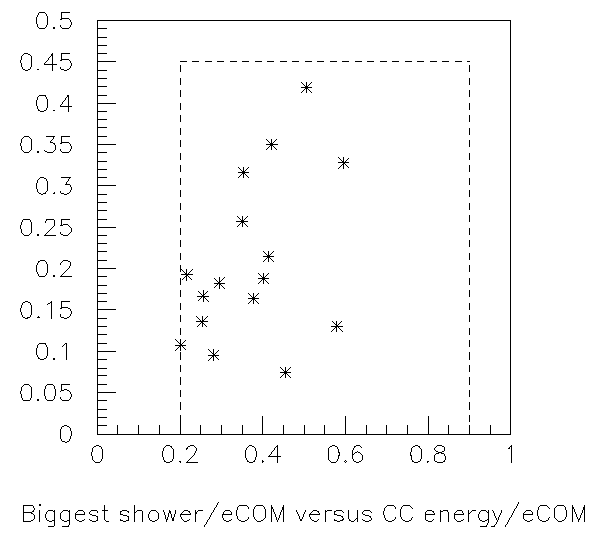
\includegraphics[width=0.9\linewidth]{cascade_still_missing3_tt.pdf}

    \end{center}
  \end{minipage}
\end{tabular}


\end{document}
